% Gemini theme
% https://github.com/anishathalye/gemini
%
% We try to keep this Overleaf template in sync with the canonical source on
% GitHub, but it's recommended that you obtain the template directly from
% GitHub to ensure that you are using the latest version.

\documentclass[final]{beamer}

% ====================
% Packages
% ====================

\usepackage[T1]{fontenc}
\usepackage{lmodern}
\usepackage[size=custom,width=120,height=74,scale=1.0]{beamerposter}
\usetheme{gemini}
\usecolortheme{gemini}
\usepackage{graphicx}
\usepackage{booktabs}
\usepackage{tikz}
\usepackage{pgfplots}

% ====================
% Lengths
% ====================

% If you have N columns, choose \sepwidth and \colwidth such that
% (N+1)*\sepwidth + N*\colwidth = \paperwidth
\newlength{\sepwidth}
\newlength{\colwidth}
\setlength{\sepwidth}{0.020\paperwidth}
\setlength{\colwidth}{0.3\paperwidth}

\newcommand{\separatorcolumn}{\begin{column}{\sepwidth}\end{column}}

% ====================
% Title
% ====================

\title{A Novel Model of Meta-populations in Point-Patch Habitats: Climate Change Effects on Mexican Free-Tailed Bats}

\author{Kapil Khanal,  \and Neelima Pandey, \and N'dri Diby }

\institute[shortinst]{Winona State University }


% ====================
% Body
% ====================

\begin{document}

\begin{frame}[t]
\begin{columns}[t]
\separatorcolumn

\begin{column}{\colwidth}

  \begin{block}{Introduction}
We are interested in analyzing how the spatial distribution, dispersal rates, and carrying capacities of caves affect equilibrium (long-term steady-state) populations of Mexican free-tailed bat (\textit {Tadarida brasiliensis mexicana}(Tbm) demographics throughout their year long life cycle. We derive equations which track the demographics of the tbm during dispersal stages in and around the caves.
\begin{figure}
      \centering
      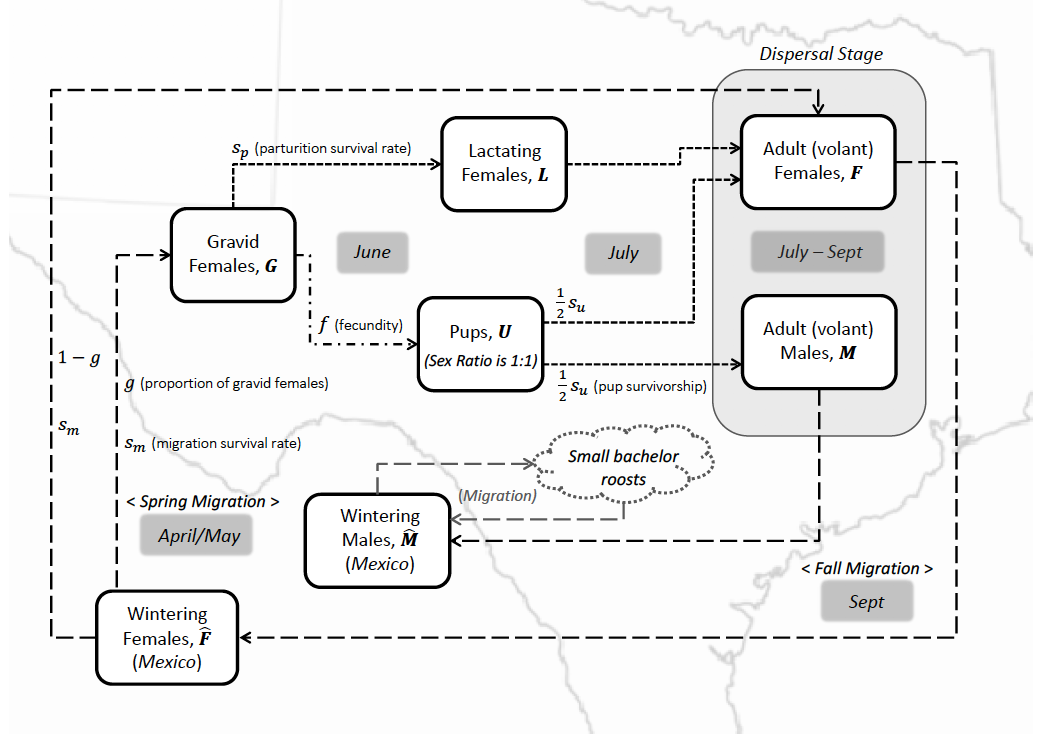
\includegraphics[width = 12cm,length = 14cm]{life-cycle}
      \caption{Mexican free tailed tbm lifecycle.}
      \end{figure}
  \end{block}
  \begin{block}{Integrodifference Model}
 We construct a model of a metapopulation in a point-patch habitat (maternity caves in Texas) in which bats use olfactory gradients to find new patches (caves) upon dispersing. Population demographics are modeled by a logistic growth model for bats in maternity caves $i=1, 2, ..., N$ on day n throughout the dispersal stage where pop.growth rates $r_i$ and carrying capacity $C_i$ are climate dependent.
\begin{equation}
    P_i(n + 1) = P_i(n) + r_i \cdot P_i(n)\left(1-\frac{P_i(n)}{C_i}\right) 
\end{equation}
    \begin{itemize}
      \item  We assume that the birth rate and carrying capacity of a cave (and immediately surrounding area) increases with local annual mean temperature as well as with annual rainfall
    \end{itemize}
    At Dusk bats forage and disperse (on a 1-dimensional landscape) according to a probability distribution $K_i(x)$, called the \textbf{dispersal kernel}, with parameters that depend on  climate conditions near each cave. We use  \textbf{Laplace Distribution} as dispersal Kernel.
\begin{equation}
    K_i(x) =
\frac{1}{2d_i}\cdot e^{\frac{-|x|}{d_i}}
\end{equation}
where $d_i$ is the climate-dependent mean dispersal distance.
To obtain the total density of tbm that dispersed from all caves, denoted by $B(x)$, we add the densities from all caves,
\begin{equation}
    B(x) = P_1(n)K_1(x-x_1) + P_2(n)K_2(x-x_2) .... + P_N(n)K_N(x-x_N):
\end{equation}
  \begin{figure}
      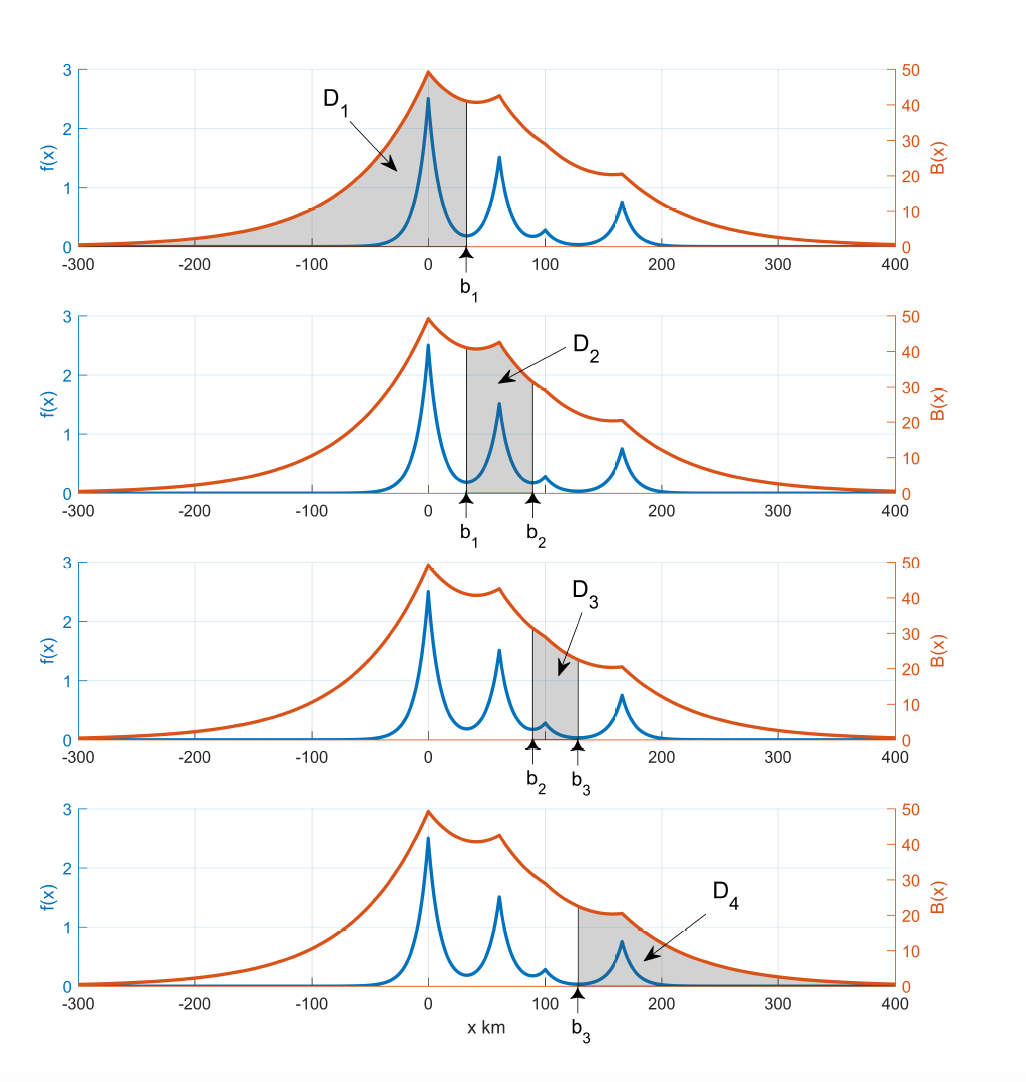
\includegraphics[width = 13cm]{one-dim.png}
      \caption {Minimums of $f$ are denoted by $b_i$, each of which forms the boundary between the region in which olfactory cue concentration gradients(\textit{order cue function}) lead tbm to cave $i$ and the
region in which they lead tbm to cave $i + 1$. The total number of tbm attracted to cave $i$ on day $n$, denoted by $Di(n)$, is the area under the bat density curve $B(x)$}
    \end{figure}
  \end{block}

  
\end{column}

\separatorcolumn

\begin{column}{\colwidth}


  \begin{block}{Extension to \textit{2}-Dimensional Landscape}
  \begin{alertblock}{
 Consider a set of $N$ caves located at points $(x_1; y_1),
 ... (x_N, y_N) $ on the $xy$-plane. Using a Bivariate Laplace distribution as dispersal kernel,
 $$K_i(x,y) =
\frac{1}{2\pi d_i^2}\cdot e^{ -\frac{\sqrt{x^2 + y^2}}{d_i}}
 $$
 we modify ($3$) as
$$
     B(x,y) = P_1(n)K_1(x-x_1,y-y_1) .....P_N(n)K_N(x-x_n,y-y_n)
     $$
 
}
  \end{alertblock}

\begin{figure}
   \hfill
\subfigure{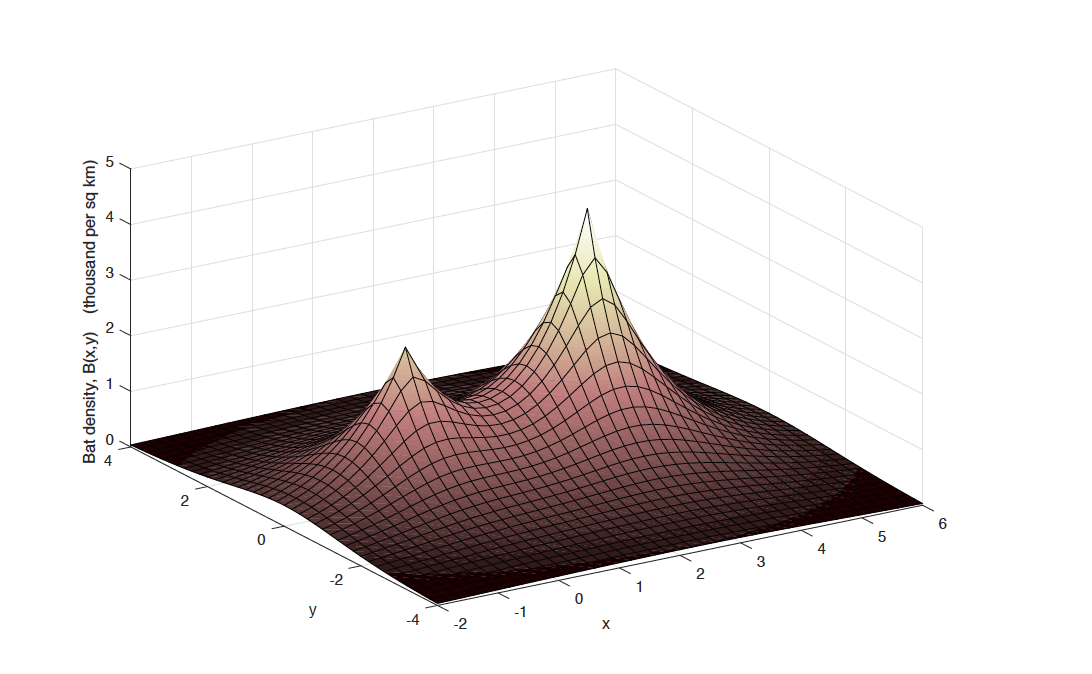
\includegraphics[width = 17cm]{two-dim}}
\hfill
\subfigure{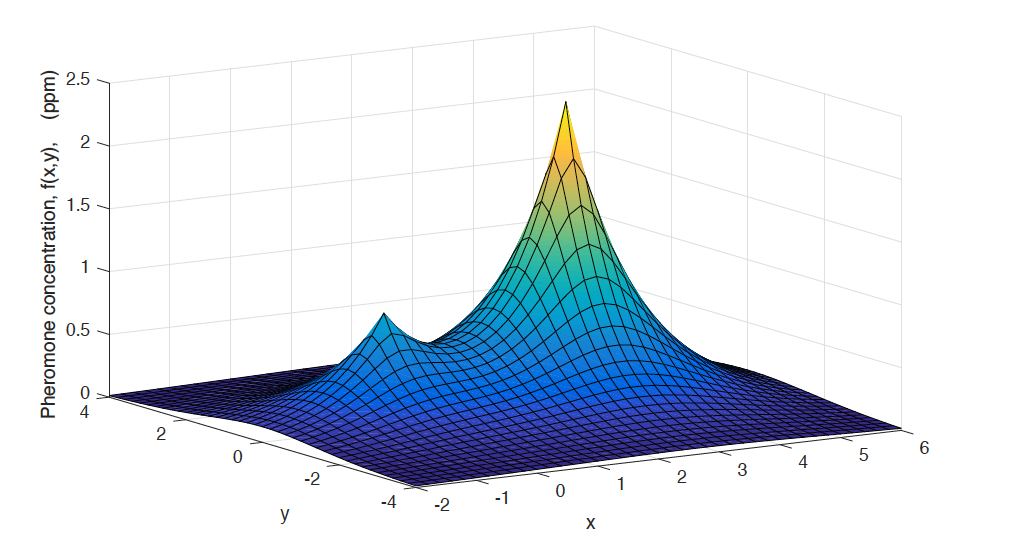
\includegraphics[width=17cm]{phero-mon.png}}
\hfill
\caption{\textit{ $B(x, y)$ across $2$-dimension},     \textit{Odor concentration function $f(x, y)$ across $2$-dimension}}
 \end{figure}
 
 \begin{figure}
 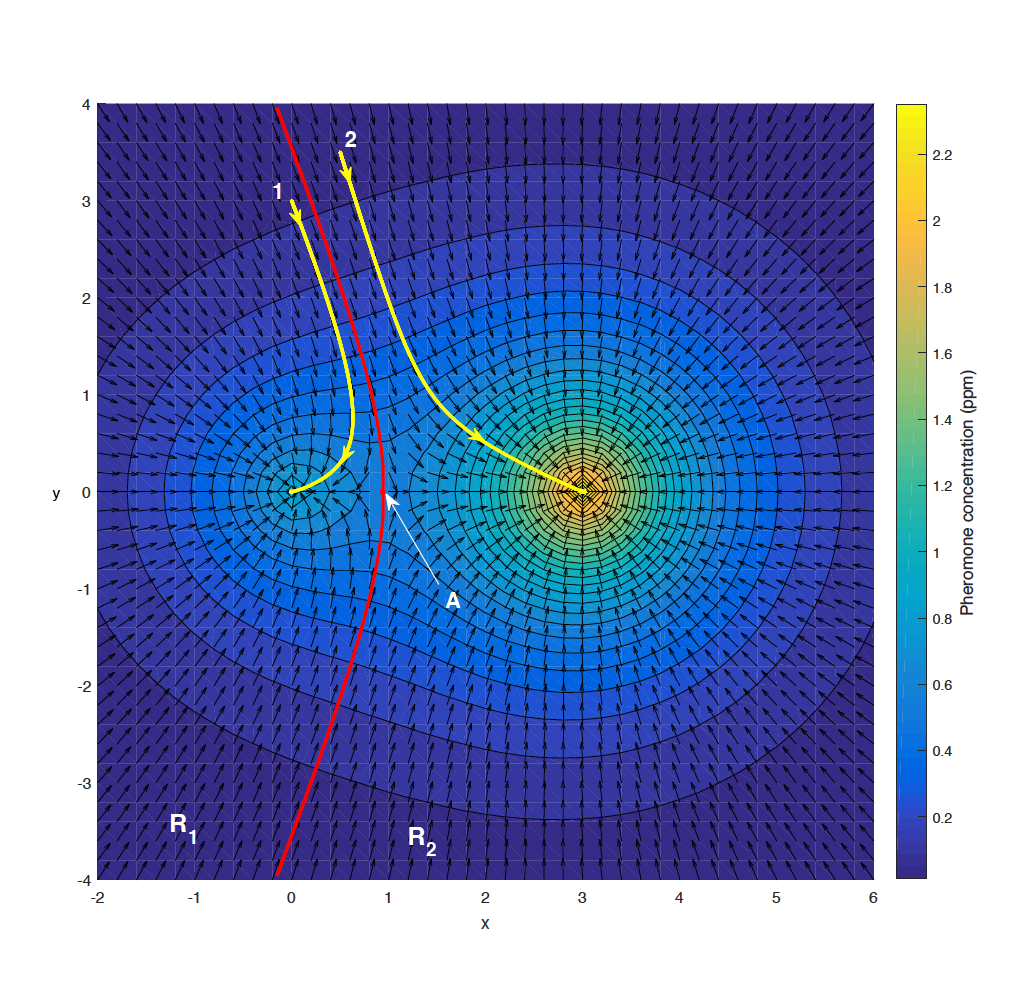
\includegraphics[width = 21cm]{contour.png}
 \caption{Gradient vector field $f(x; y)$ , 
 for caves with two example bat trajectories (yellow
curves) in cave finding after foraging.  The boundary separating the region, $R_1$, in which tbm return to cave $1$ from the
region, $R_2$, in which tbm return to cave $2$ is called a separatrix (red curve)}
 \end{figure}
 With an arbitrary number of caves ($N$), the gradient field will partition the plane into $N$ regions,
$R_1, R_2, ... ,R_N,$ in which tbm return to caves $1, 2, ..., N$ respectively. The total number of tbm attracted to cave $i$ after foraging on day $n$ is determined by the total density of tbm in region $R_i$,
\newcommand{\Int}{\int\limits}
\begin{equation}
    D_i(n) = \Int_ {}^{}\Int_{R_i}^{}B(x,y) \,dA
\end{equation}
  \end{block}
\end{column}

\separatorcolumn

\begin{column}{\colwidth}

  \begin{block}{Model Parameterization, Simulation, and Prediction}
    \heading{$4$-Cave Model Simulation}
we plan to parameterize the model with data gathered by remote sensors that track daily populations emerging from caves.  This will be done in collaboration with bat researcher \textit{Laura Kloeppe}. We also investigate the effect of climate conditions on equilibrium populations.We provide a brief expository analysis of the $4$-Cave model in $1$-dimension here.
 \begin{figure}
 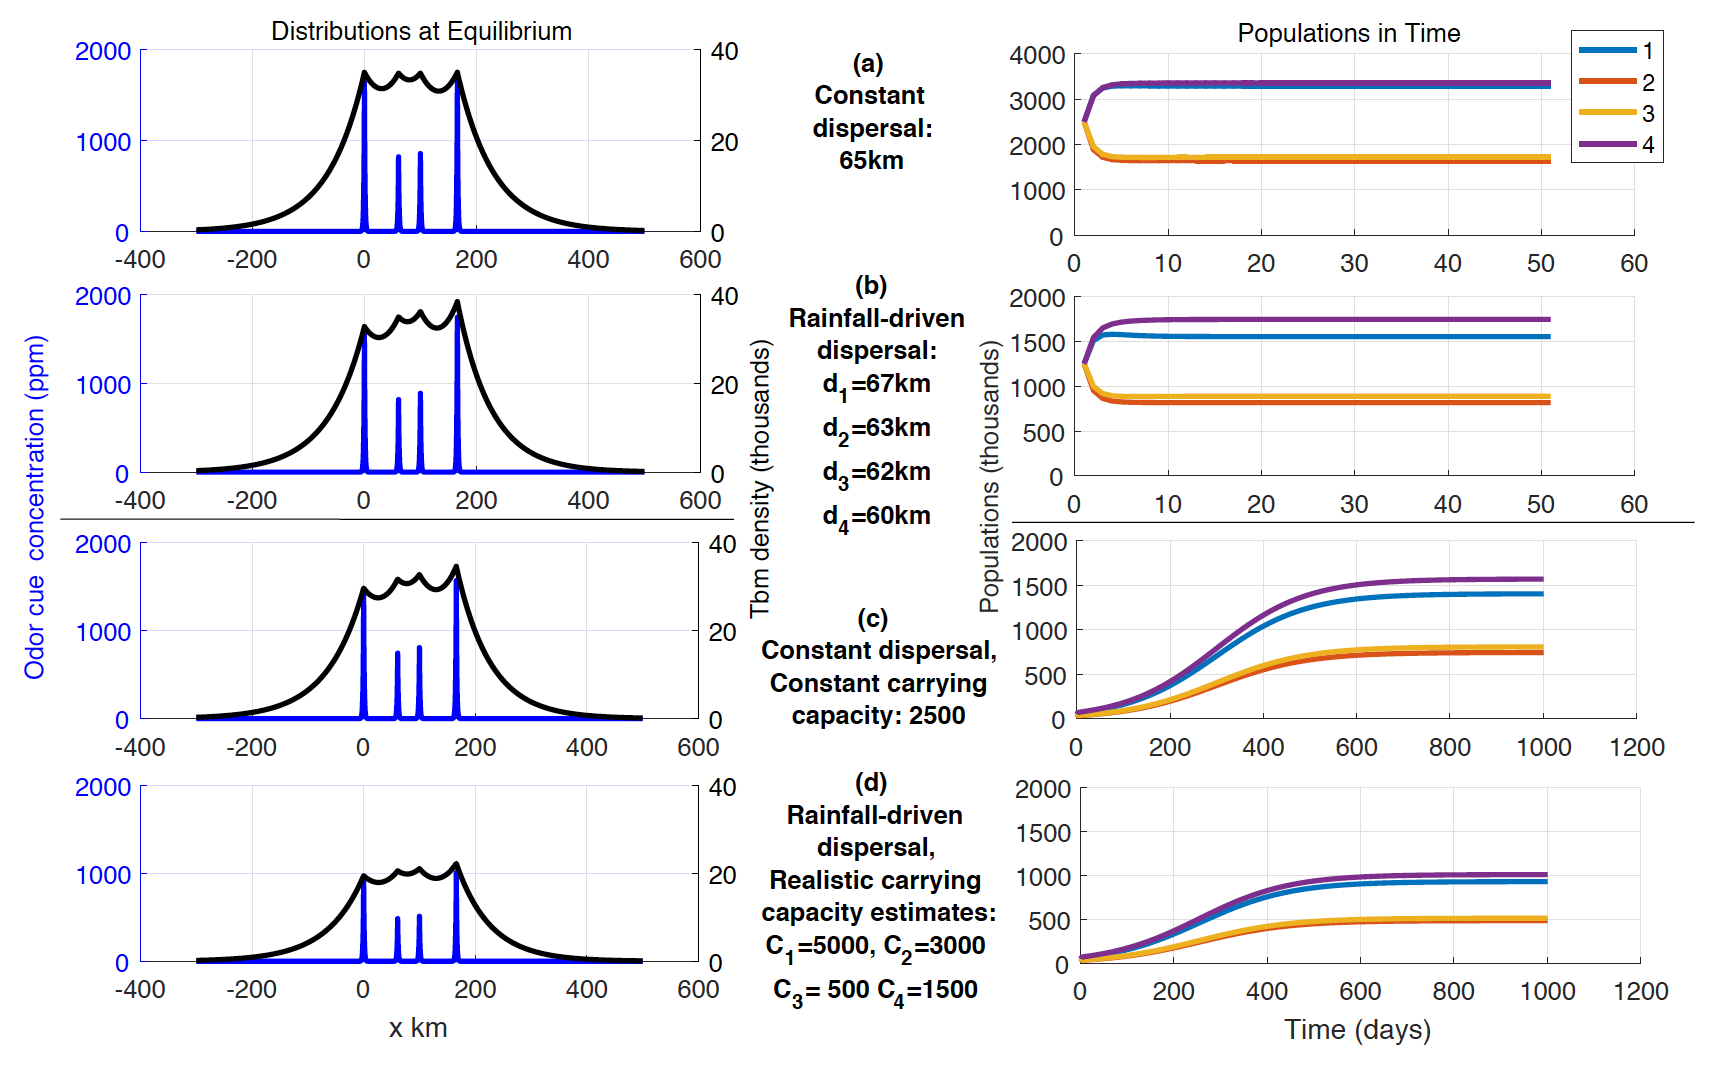
\includegraphics[width = 30cm]{fullmodel.png}
 \caption{Simulation of the full model with constant dispersal rate (65 km) and carrying capacity (2.5
million) for closely situated caves (a), and caves significantly far apart (b). Dispersal is more of a factor than
carrying capacity in determining equilibrium populations when caves are close together. If caves are far
apart, the system tends more toward the carrying capacities than the intrinsic dispersal-driven equilibrium
populations.}
 \end{figure}
  \end{block}
  \begin{block}{Equilibrium Analysis }
    Simulations give good qualitative insight into the spatiotemporal dynamics of bat
 populations in point-patch habitats. However,our long-term goal is to derive predictions of equilibrium is to use the real data from sensors to derive model for equilibrium populations in terms of spatial distribution of caves, as well as climate-dependant dispersal rates, birth rates, and carrying capacities. We can then use such models to analyze the effect of  climate change on long term (equilibrium) populations. 
  \end{block}
  \begin{block}{Acknowledgements}
   We would like to thank Dr. Jacob Duncan(Winona State University,Mathematics and Statistics) and Laura Kloepper (Saint Mary's College, Notre Dame Biology) for helping us with the analysis.
  \end{block}
\end{column}

\end{columns}
\end{frame}
\end{document}
